\documentclass[hidelinks,12pt]{article}
\usepackage[left=0.25cm,top=1cm,right=0.25cm,bottom=1cm]{geometry}
%\usepackage[landscape]{geometry}
\textwidth = 20cm
\hoffset = -1cm
\usepackage[utf8]{inputenc}
\usepackage[spanish,es-tabla]{babel}
\usepackage[autostyle,spanish=mexican]{csquotes}
\usepackage[tbtags]{amsmath}
\usepackage{nccmath}
\usepackage{amsthm}
\usepackage{amssymb}
\usepackage{mathrsfs}
\usepackage{graphicx}
\usepackage{subfig}
\usepackage{standalone}
\usepackage[outdir=./Imagenes/]{epstopdf}
\usepackage{siunitx}
\usepackage{physics}
\usepackage{color}
\usepackage{float}
\usepackage{hyperref}
\usepackage{multicol}
%\usepackage{milista}
\usepackage{anyfontsize}
\usepackage{anysize}
%\usepackage{enumerate}
\usepackage[shortlabels]{enumitem}
\usepackage{capt-of}
\usepackage{bm}
\usepackage{relsize}
\usepackage{placeins}
\usepackage{empheq}
\usepackage{cancel}
\usepackage{wrapfig}
\usepackage[flushleft]{threeparttable}
\usepackage{makecell}
\usepackage{fancyhdr}
\usepackage{tikz}
\usepackage{bigints}
\usepackage{scalerel}
\usepackage{pgfplots}
\usepackage{pdflscape}
\pgfplotsset{compat=1.16}
\spanishdecimal{.}
\renewcommand{\baselinestretch}{1.5} 
\renewcommand\labelenumii{\theenumi.{\arabic{enumii}})}
\newcommand{\ptilde}[1]{\ensuremath{{#1}^{\prime}}}
\newcommand{\stilde}[1]{\ensuremath{{#1}^{\prime \prime}}}
\newcommand{\ttilde}[1]{\ensuremath{{#1}^{\prime \prime \prime}}}
\newcommand{\ntilde}[2]{\ensuremath{{#1}^{(#2)}}}

\newtheorem{defi}{{\it Definición}}[section]
\newtheorem{teo}{{\it Teorema}}[section]
\newtheorem{ejemplo}{{\it Ejemplo}}[section]
\newtheorem{propiedad}{{\it Propiedad}}[section]
\newtheorem{lema}{{\it Lema}}[section]
\newtheorem{cor}{Corolario}
\newtheorem{ejer}{Ejercicio}[section]

\newlist{milista}{enumerate}{2}
\setlist[milista,1]{label=\arabic*)}
\setlist[milista,2]{label=\arabic{milistai}.\arabic*)}
\newlength{\depthofsumsign}
\setlength{\depthofsumsign}{\depthof{$\sum$}}
\newcommand{\nsum}[1][1.4]{% only for \displaystyle
    \mathop{%
        \raisebox
            {-#1\depthofsumsign+1\depthofsumsign}
            {\scalebox
                {#1}
                {$\displaystyle\sum$}%
            }
    }
}
\def\scaleint#1{\vcenter{\hbox{\scaleto[3ex]{\displaystyle\int}{#1}}}}
\def\bs{\mkern-12mu}


\title{Tema 2 - Lista de ejercicios a cuenta - Solución\\ \large{Matemáticas Avanzadas de la Física}\vspace{-3ex}}
\author{M. en C. Gustavo Contreras Mayén}
\date{ }
\begin{document}
\vspace{-4cm}
\maketitle
\fontsize{14}{14}\selectfont

\section{Presentación 1. Introducción a las EDP.}

Describe el tipo de ecuación y las regiones en las que es de tipo hiperbólica, parabólica y/o elíptica. Recuerda que debes de justificar el por qué de tu respuesta, es decir, deberás de realizar las operaciones y cálculos necesarios para tu respuesta.

\begin{enumerate}[label=\alph*)]
\item \Large{$u_{xx} - u_{xy} - 2 \, u_{yy} = 0$}
\item \Large{$u_{xx} + 2 \, u_{xy} + u_{yy} = 0$}
\item \Large{$2 \, u_{xx} + 4 \, u_{xy} + 3 \, u_{yy} - 5 \, u = 0$}
\item \Large{$u_{xx} + 2 \, x \, u_{xy} + u_{yy} + (\cos x \, y) \, u_{x} - u = 0$}
\item \Large{$y \, u_{xx} - 2 \, u_{xy} + e^{x} \, u_{yy} + u - 3 = 0$}
\item \Large{$e^{x y} \, u_{xx} + (\sinh x) \, u_{yy} + u = 0$}
\item \Large{$x \, u_{xx} + 2 \, x \, u_{xy} - y \, u_{yy} = 0$}
\item \Large{$x \, u_{xx} + 2 \, x \, u_{xy} + y \, u_{yy} = 0$}
\end{enumerate}

\subsection{Solución.}

\begin{enumerate}[label=\alph*)]
\item {\Large{$u_{xx} - u_{xy} - 2 \, u_{yy} = 0$}}
\\
Se tiene que: $A = 1$, $B = -1$, $C = -2$, entonces:
\begin{align*}
B^{2} -  4 \, A \, C = (-1)^{2} - 4 (1)(-2) = 1 + 8 = 9 > 0
\end{align*}
Por lo tanto, la EDP es \underline{hiperbólica}.
\item {\Large{$u_{xx} + 2 \, u_{xy} + u_{yy} = 0$}}
\\
Se tiene que: $A = 1$, $B = 2$, $C = 1$, entonces:
\begin{align*}
B^{2} -  4 \, A \, C = (2)^{2} - 4 (1)(1) = 4 - 4 = 0
\end{align*}
Por lo tanto, la EDP es \underline{parabólica}.
\item {\Large{$2 \, u_{xx} + 4 \, u_{xy} + 3 \, u_{yy} - 5 \, u = 0$}}
\\
Se tiene que: $A = 2$, $B = 4$, $C = 3$, entonces:
\begin{align*}
B^{2} -  4 \, A \, C = (4)^{2} - 4 (2)(3) = 16 - 24 = -8 < 0
\end{align*}
Por lo tanto, la EDP es \underline{elíptica}.
\item {\Large{$u_{xx} + 2 \, x \, u_{xy} + u_{yy} + (\cos x \, y) \, u_{x} = 0$}}
\\
Se tiene que: $A = 1$, $B = 2 \, x$, $C = 1$, entonces:
\begin{align*}
D = B^{2} -  4 \, A \, C = (2 \, x)^{2} - 4 (1)(1) = 4 \, x^{2} - 4
\end{align*}
Por lo que en este caso hay que revisar como se comporta el discriminante en relación al dominio de la variable $x$:
\begin{align*}
\begin{cases}
\mbox{En } x = 0, D = 4 (0)^{2} - 4 = - 4 < 0 & \therefore \text{ la EDP es \underline{elíptica}} \\
\mbox{En } x < 1, x > 1, D = 4 \, x^{2} - 4 > 0 & \therefore \text{ la EDP es \underline{hiperbólica}} \\
\mbox{En } x = \pm 1, D = 4 (\pm 1)^{2} - 4 = 0 & \therefore \text{ la EDP es \underline{parabólica}} \\
\end{cases}
\end{align*}
\item {\Large{$y \, u_{xx} - 2 \, u_{xy} + e^{x} \, u_{yy} + u - 3 = 0$}}
\\
Se tiene que $A = y$, $B = -2$, $C =e^{x}$, entonces:
\begin{align*}
D = B^{2} - 4 \, A \, C = (-2)^{2} - 4 \, y \, e^{x} = 4 - 4 \, y \, e^{x}
\end{align*}
Que tendremos que revisar nuevamente, pero ahora tanto para el dominio de la variable $y$ como para la variable $x$:
\par
La función $e^{x}$ siempre es positiva en $-\infty < x < \infty$, por lo que el tipo de EDP dependerá del dominio de la variable $y$:
\begin{align*}
\begin{cases}
\mbox{En } y = 0, D = 4 > 0 & \therefore \mbox{ la EDP es parabólica} \\
\mbox{En } y = 1, x = 0, D = 0 & \therefore \mbox{ la EDP es parabólica} \\
\mbox{En } y < 1 \setminus \left\{ 0 \right\}, D > 0 & \therefore \mbox{ la EDP es hiperbólica} \\
\mbox{En } y > 1, D < 0 & \therefore \mbox{ la EDP es elíptica} \end{cases}
\end{align*}
\item {\Large{$e^{x y} \, u_{xx} + (\sinh x) \, u_{yy} + u = 0$}}
\\
Se tiene que: $A = e^{x y}$, $B = 0$, $C = \sinh x$, por lo que el discriminante resulta ser:
\begin{align*}
D = B^{2} - 4 \, A \, C = - 4 \, e^{x y} \, \sinh x
\end{align*}
Tendremos que revisar con cuidado, cómo se comporta cada función en los respectivos dominios, nos apoyaremos con las gráficas de las funciones:
\begin{figure}[H]
    \centering
    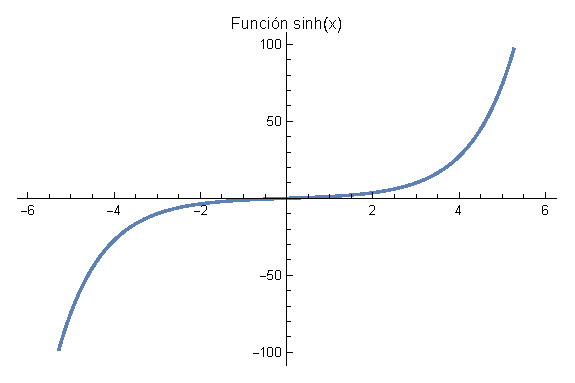
\includegraphics[scale=1]{Imagenes/Ejercicio_Plot_01.eps}
    \caption{La gráfica de la función $\sinh x$.}
    \label{fig:plot_01_sinhx}
\end{figure}
Vemos de la figura (\ref{fig:plot_01_sinhx}) que la función $\sinh x$ es positiva para $x > 0$, es negativa para $x < 0$ y en $x = 0$, la función se anula.
\begin{figure}[H]
    \centering
    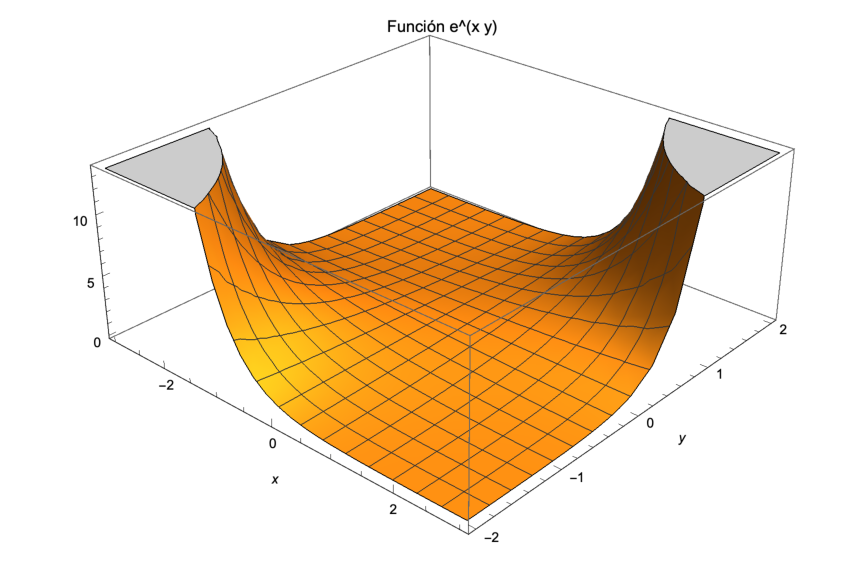
\includegraphics[scale=1]{Imagenes/Ejercicio_Plot_02.eps}
    \caption{La gráfica de la función $\exp(x \, y)$.}
    \label{fig:plot_02_exp_xy}
\end{figure}
De la figura (\ref{fig:plot_02_exp_xy}) tenemos que la función siempre es positiva, de hecho $\exp(x \, y) > 1, \forall \, x, y \in \mathbb{R}$. Por lo que tenemos que revisar con cuidado el producto de las dos funciones: $D = \exp(x \, y ) \, \sinh x$:
\begin{figure}[H]
    \centering
    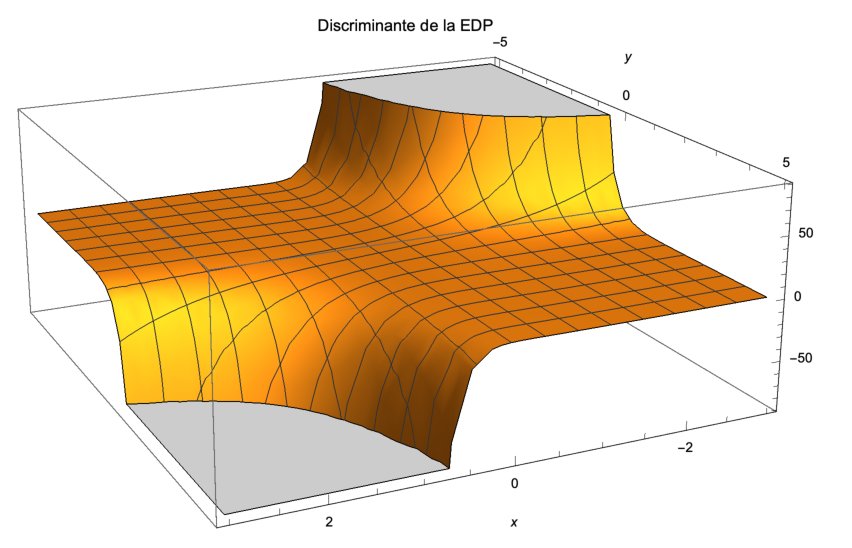
\includegraphics[scale=1]{Imagenes/Ejercicio_Plot_03.eps}
    \caption{La gráfica de la función $\exp(x \, y) \, \sinh x$.}
    \label{fig:plot_03_exp_xy_sinhx}
\end{figure}
\begin{align*}
\begin{cases}
\mbox{En } x = 0, \, \forall \, y \in \mathbb{R}, D = 0 \mbox{ , por lo tanto la EDP es \underline{parabólica}}. \\
\mbox{Para } x > 0, \, y > 0, D < 0 \mbox{ , por lo tanto la EDP es \underline{elíptica}}. \\
\mbox{Para } x < 0, \, y < 0, D > 0 \mbox{ , por lo tanto la EDP es \underline{hiperbólica}}. \\
\end{cases}
\end{align*}
\item $x \, u_{xx} + 2 \, x \, u_{xy} - y \, u_{yy} = 0$ \label{eq:inciso_07}
Se tiene que: $A = x$, $B = 2 \, x$, $C = -y$, por lo que el discriminante resulta ser:
\begin{align*}
D = B^{2} - 4 \, A \, C = (2 \, x)^{2} - 4 \, (x) (-y) = 4 x^{2} + 4 \, x \, y
\end{align*}
Nuevamente hay que revisar con cuidado, cómo se comporta cada función en los respectivos dominios, por lo que también nos apoyamos con la gráfica del discriminante:
\begin{figure}[H]
    \centering
    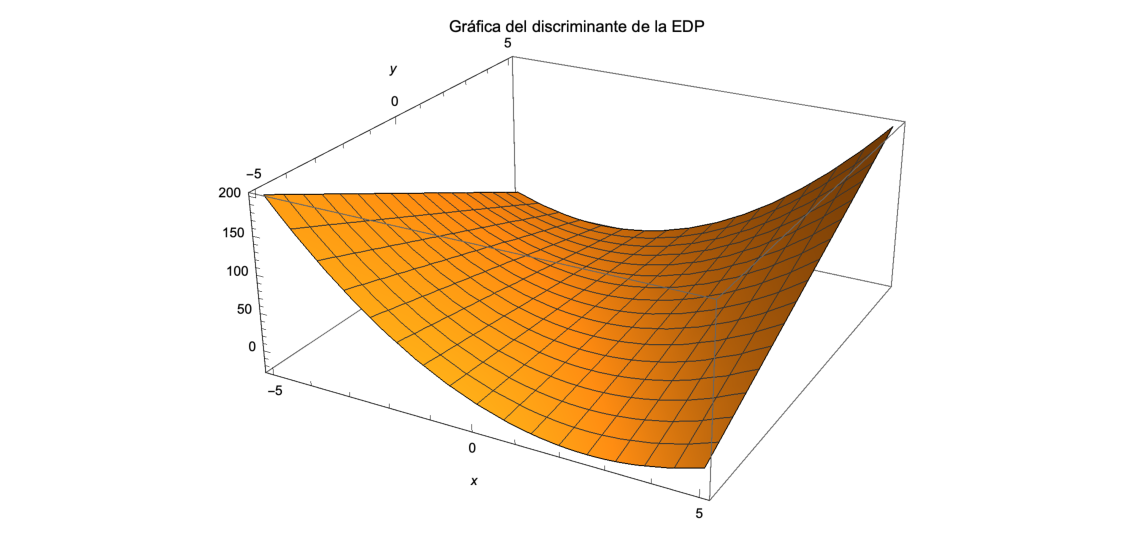
\includegraphics[scale=0.85]{Imagenes/Ejercicio_Plot_04.eps}
    \caption{La gráfica de la función $4 x^{2} + 4 \, x \, y$.}
    \label{fig:plot_04_4x2+4xy}
\end{figure}
De la figura (\ref{fig:plot_04_4x2+4xy}) encontramos que para los puntos $x = 0$, $y = 0$, el valor del discriminante es $D = 0$, mientras que para todos los puntos de $x$, $y$ (excepto en el origen), el discriminante es $D > 0$, así que ya podemos clasificar la EDP de la siguiente manera:
\begin{align*}
\begin{cases}
\mbox{En } x = 0 \, y = 0, \, D = 0, \mbox{ por lo que la EDP es \underline{elíptica.}} \\
\forall \, x \setminus \left\{ 0 \right\}, \, \forall \, y  \setminus \left\{ 0 \right\}, \, D > 0, \mbox{ por lo que la EDP es \underline{hiperbólica.}}
\end{cases}
\end{align*}
\item $x \, u_{xx} + 2 \, x \, u_{xy} + y \, u_{yy} = 0$
\\
Este ejercicio es parecido al inciso (\ref{eq:inciso_07}, solo que el signo del tercer sumando es positivo en este caso. Veamos cómo queda el determinante: se tiene que: $A =  x$, $B = 2 , x$, $C = y$, por lo que:
\begin{align*}
D = B^{2} - 4 \, A \, C = (2 \, x)^{2} - 4 \, (x) (y) = 4 x^{2} - 4 \, x \, y
\end{align*}
Revisemos la gráfica para tener una idea de cómo es el determinante:
\begin{figure}[H]
    \centering
    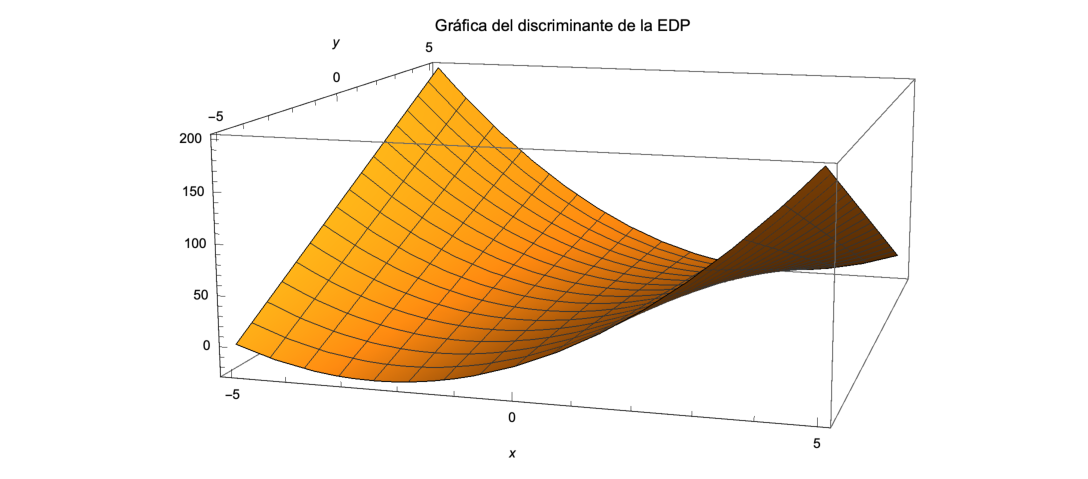
\includegraphics[scale=0.85]{Imagenes/Ejercicio_Plot_05.eps}
    \caption{La gráfica de la función $4 x^{2} - 4 \, x \, y$.}
    \label{fig:plot_04_4x2-4xy}
\end{figure}
Tenemos en una primera revisión que la gráfica del determinante parecería que es positiva para valores tanto positivos como negativos de $x$ e $y$, pero si analizamos con cuidado el determinante, revisemos en qué puntos se hace menor que cero:
\begin{align*}
D &= 4 x^{2} - 4 \, x \, y < 0 \\[0.5em]
&4 \, x^{2} < 4 \, x \, y \\[0.5em]
&x^{2} < x \, y \\[0.5em]
&\pm \, x < \sqrt{x \, y}
\end{align*}
Entonces en este conjunto de puntos el determinante es menor que cero, mientras que el resto de los valores (excepto $x = 0$), el determinante se hace positivo, así tenemos que:
\begin{align*}
\begin{cases}
\mbox{En } x = 0, \forall \, y \in R , D = 0, \mbox{ por lo que la EDP es \underline{parabólica.}} \\
\mbox{Para } \Psi = \pm \, x < \sqrt{x \, y} \setminus \left\{ 0 \right\}, D < 0, \mbox{ por lo que la EDP es \underline{elíptica.}} \\
\mbox{Para } \forall \, x, y \in \mathbb{R} \setminus \left\{ \Psi \right\}, D > 0, \mbox{ por lo que la EDP es \underline{hiperbólica.}}
\end{cases}
\end{align*}
\end{enumerate}
\end{document}